\section{Natural numbers as grammar}
Climbing could find many routes, even go in cycles, but 
evaluating a formula was a precise algorithm without ambiguity.
The reason was that we had a tree.  Trees have unique paths between 
any two vertices. So if we start at the bottom we have a unique direction to 
reach the top.  Recursion on trees is so special it has a special name:
\emph{traversing} the tree.  

Parsing grammars in natural language is not always that
uniform.  A simplistic English grammar will often parse into cycles.
\begin{center}
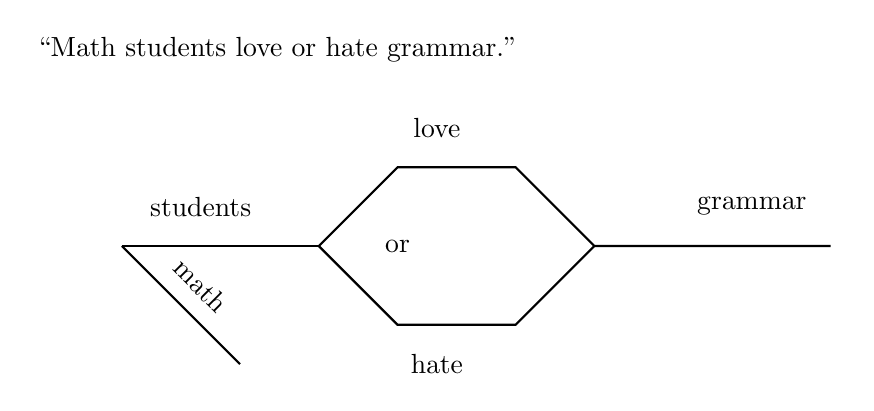
\begin{tikzpicture}
    \node[text width=4in] at (0,2) {``Math students love or hate grammar.''};
    \node at (-3,0) {students};
    \node[rotate=-45] at (-3,-1) {math};
    \node at (-0.5,-0.5) {or};
    \node at (0,1) {love};
    \node at (0,-2) {hate};
    \node at (4,0) {grammar};

    \draw[thick] (-4,-0.5) -- ++(2.5,0);
    \draw[thick] (-4,-0.5) -- ++(1.5,-1.5);
    \draw[thick] (-1.5,-0.5) -- ++(1,1) -- ++(1.5,0) -- ++(1,-1) -- ++(3,0);
    \draw[thick] (-1.5,-0.5) -- ++(1,-1) -- ++(1.5,0) -- ++(1,1);

\end{tikzpicture}
\end{center}
In mathematics two paths to the same place are said to be a relation, 
they are related.  So systems that have no cycles, i.e.\ trees, are 
free of relations, or simply \emph{free}.  In time we will come to see 
that every algebraic structure can be constructed from a free 
structure with the possible addition of relations.

\begin{remark}
What is free in this case 
is the grammar we used for arithmetic formulas.  
For example $7(7+3)(7+3)$ renders the same result 700, and nearly 
by the same steps.  Yet, if we diagrammed that formula as 
parse tree it would quite different because we could for example 
multiply $7\cdot 10$ then by $10$ rather than squaring $10$.
Having two formulas that reduce to the same value is not the same 
as a relation in the grammar.  It is said that the \emph{syntax} is 
different but the \emph{semantics} is the same.
\end{remark}

\index{context-free}
That we got a tree in math formulas means we have a rather boring grammar, 
what Chompsky's \emph{Syntactic Structure} calls
\emph{context-free} grammars.\footnote{
    If an algebraist starts a talk with a story that ``...It was thought  all natural 
    languages were context-free until some obscure dialect in the alps or Africa was found...'', 
    then tune out until they return to equations.  
    Linguist never had such illusions. Even english is not context-free, read  James Higginbotham.} 
Don't be too disheartened.  Virtually every programming language has a 
context-free grammar and programs can communicate a lot of hefty ideas. 
Let us begin with an example.

\subsection{Introducing counting}
Early history (early childhood) is counting.  Count 
pebbles or beads and give the patterns names
\begin{center}
    $0\defeq$ \underline{\hspace{5mm}}, 
    $1\defeq$ \StrokeOne,
    $2\defeq$ \StrokeTwo,
    $3\defeq$ \StrokeThree,
    $4\defeq$ \StrokeFour,
    $5\defeq$ \StrokeFive,...
\end{center}
``0'' might have been chosen as the shape left by removing the last pebble from a sand 
table leaving behind zero pebbles.

It struck Giuseppe Peano in the early 1900's that tallies 
would be easier to get right mathematically than digits. With the following two rules
Peano introduced the natural numbers to the formalism of math.
\begin{quote}
    \textit{
    $N_0$ vale ``numero'', et es nomen commune de 0,1,2, etc.\\
    $0$ $\to$  ``zero''\\
    $+$ $\to$ ``plus''.  Si $a$ es numero, $a+$ indica ``numero sequente $a$''.
    }
\end{quote}
% It is fitting that the Italian is in italics.
(See G. Peano \emph{Formulaire de mathematiques.~I-V}, p.27.)
Replacing $+$ with \StrokeOne ~(and equating \StrokeFive$\defeq$\StrokeFour~\StrokeOne),
Peano's model of numbers is simply the grammar of tallies.

Today notation has evolved.  These numbers are now almost always designated as
\emph{natural numbers} and denoted $\mathbb{N}$.  Instead of $a+$ we now 
often write $S(k)$ of the ``successor'' to the natural number $k$.  Other 
authors use $a++$ or $++a$ to mimic trends in programming languages.  

We mentioned Peano was merely recording a grammar.  Today we write grammars with 
list of rules, called \emph{production rules}.  Some rules are to specify 
what makes up the alphabet of symbols in our grammar.  For Peano, $0$ and $S$
are the complete alphabet.  So we may write either $0$ on its own, or 
we may pre-pend the symbol $S$ to any existing natural number.  
Each rule is given a name called a \emph{token} (or \emph{tag}) and 
denoted \code{<Name>}. Since the Walrus
$\defeq$ is our assignment of variables (more on this later), 
we use the ``astonished Walrus'' $::=$
as assignment of production rules.   Taken together the grammar is this.
\begin{center}
\begin{gcode}[]
<Nat> ::= 0 
<Nat> ::= S <Nat>
\end{gcode}
\end{center}
In the first rule we are told \code{0} is a natural number, denoted
\code{0:Nat}. We say that the grammar \emph{accepts} \code{0} because it matched
some production rule.  In the second rule if we encounter an \code{S} it must be
followed by an \emph{already known} natural number.  So \code{S0:Nat} but
\code{0S} would not be accepted as it is not found as a production rule, we say
the grammar \emph{rejects} \code{0S}.  Going forward we will start write 
$S(k)$, or $S~k$, where $k:\mathbb{N}$.

Graphically we can render accepted words with parse trees, in this case with no branches.
\begin{center}
    \begin{tikzpicture}
        \node (0) at (0,0) {0};
        \node (1) at (3,0) {S0};
        \node (2) at (6,0) {SS0};
        \draw[thick,->] (0) edge["S"] (1);
        \draw[thick,->] (1) edge["S"] (2);
    \end{tikzpicture}
\end{center}

\begin{definition}
A production rule that appears more than once is called \emph{inductive}.
An accepted short hand for inductive productions rules is to name it once 
and separate the cases by $\mid$, for instance,
\begin{center}
\begin{gcode}[]
<Nat> ::= 0 | S <Nat>
\end{gcode}
\end{center}
\end{definition}



\begin{remark}
    The power of the ``already known'' clause of the rules is to prevent ambiguity 
    with terms like $n=$\code{SSS....} where the \code{S} continue forever.
    See if we remove on \code{S} form $n$, the string is the same as $n$.
    Since we are engaged in deciding if $n$ is a natural number and its substring 
    is $n$, it is not of the form \code{S k} for \code{k:Nat}.  Hence the grammar 
    rejects such an $n$.  Grammar's like these are called \emph{primitive recursive}
    meaning that the recursion can only depend backwards 
    in history.
\end{remark}

We do well to acknowledge inductive types a basic programs.
Computers understand this much.
Listing~\ref{lst:peano} shows two programs you could run today that implement Peano's idea.
There are of course many differences.  Visibly, the left-hand side 
favors mathematically minded symbolic notation and 
economizes even on parentheses in the spirit of ``$\sin x$'' notation.
Meanwhile the right-hand side favors a verbose imitation of 
natural language and prefers the $\sin(x)$ notation.  Set the differences 
aside.

\begin{lstfloat}
\begin{center}
\begin{minipage}{0.4\textwidth}
\begin{Fcode}[]
data Nat = Z 
         | S k

zero = Z
two = S (S zero)
\end{Fcode}
\end{minipage}
\hfill
\begin{minipage}{0.59\textwidth}
\begin{Pcode}[language=Sava]
class Nat
    case Zero() extends Nat
    case Next(k:Nat) extends Nat
sealed  // no more cases
zero = new Zero()
two = new Next(new Next(zero))
\end{Pcode}
\end{minipage}
\end{center}
\caption{Peano's natural numbers programmed in two different languages.}
\label{lst:peano}
\end{lstfloat}
    

Even without a deep understanding of these programs, one can 
make out the contours of Paeno's definitions.  Both use a mix of 
keywords (in blue) to tell our system to prepare a new type (or class) of data 
that will be called \code{Nat}.  Then they instruct the system 
to accept exactly two ways to make such data.
It may be some initial state, \code{Z}, respectively 
\code{Zero}, that depends on nothing;
otherwise, we must give data \code{k} of type \code{Nat},
denoted \code{k:Nat}, which will then produce new data 
\code{S k}, respectively \code{Next(k)}.


\subsection{Eliminating counting}
    
Now that we have created numbers we shall want to use them.
An obvious use of numbers in counting is to make the process 
modular and parallel.  For example we can have two separate counts 
later combined by addition.
\begin{center}
    \begin{tabular}{c|ccccc}
    ``add'' & \StrokeOne & \StrokeTwo & \StrokeThree & \StrokeFour & \StrokeFive\\
    \hline 
    \StrokeOne & \StrokeTwo & \StrokeThree & \StrokeFour & \StrokeFive & \StrokeOne \StrokeFive\\
    \StrokeTwo & \StrokeThree & \StrokeFour & \StrokeFive & \StrokeOne \StrokeFive & \StrokeTwo \StrokeFive\\
    \StrokeThree & \StrokeFour & \StrokeFive & \StrokeOne \StrokeFive & \StrokeTwo \StrokeFive & \StrokeThree \StrokeFive \\
    \StrokeFour & \StrokeFive & \StrokeOne \StrokeFive & \StrokeTwo \StrokeFive & \StrokeThree \StrokeFive & \StrokeFour \StrokeFive\\
    \StrokeFive & \StrokeOne \StrokeFive & \StrokeTwo \StrokeFive & \StrokeThree \StrokeFive & \StrokeFour \StrokeFive & \StrokeFive \StrokeFive\\
    \end{tabular}
    \hspace{1cm}
    \begin{tabular}{|c|cccccc|}
        \hline 
        + & 0 & 1 & 2 & 3 & 4 & 5\\
        \hline 
        0 & 0 & 1 & 2 & 3 & 4 & 5 \\
        1 & 1 & 2 & 3 & 4 & 5 & 6\\
        2 & 2 & 3 & 4 & 5 & 6 & 7\\
        3 & 3 & 4 & 5 & 6 & 7 & 8\\
        4 & 4 & 5 & 6 & 7 & 8 & 9\\
        5 & 5 & 6 & 7 & 8 & 9 & 10\\
    \hline
    \end{tabular}
\end{center}
Beyond a table we need some formulas.  If we have two groups $m$ and $n$ and each is either nothing 
or a successor to something else, then that leaves us with just four cases 
to consider.
\begin{align*}
    \begin{array}{|c|cc|}
        \hline 
        + & 0 & S(k)\\
        \hline 
        0 & 0 & S(k) \\
        S(\ell) & S(\ell) & S(S(\ell+k))\\
        \hline
    \end{array}
\end{align*}
As the first column does not change $m$ we can simplify this down to 2 cases.
\begin{align*}
    m+n \defeq \begin{cases} m & n=0\\ S(m+k) & n=S(k)\end{cases}
\end{align*}
Lets see this out one some examples, recalling that $1=S0$, $2=S1$, $3=S2$ and so on.
\begin{align*}
    3+2 & = S(3+1)= SS(3+0) = SS3=5.\\
    7+3 & = S(7+2) = SS(7+1) = SSS(7+0)=SSS7=10.
\end{align*}
Notice something about this process is eliminating, or consuming, 
our number $n$ in the sum $m+n$.  

And this process gives immediate significance to computation.
To use an inductive type in a program we simply run through the cases.
Programming languages allow for case-by-case analysis in numerous ways 
but most today offer some form of \emph{pattern matching} which is 
where we list the types of production rules and then attach the outcome 
for each.
\begin{lstfloat}
\begin{center}
\begin{minipage}{0.4\textwidth}
\begin{Fcode}[]
+:Nat->Nat->Nat
+ m  0    = m
+ m (S k) = + m k
\end{Fcode}
\end{minipage}
\hfill
\begin{minipage}{0.59\textwidth}
\begin{Pcode}[]
def add(m,n:Nat):Nat =
  match n with 
    Zero() => m
    Next(k)=> Next(add(m,k))
\end{Pcode}
\end{minipage}
\end{center}
\caption{Peano's addition of natural numbers programmed in two different languages.}
\label{lst:peano}
\end{lstfloat}


So in a sense our grammar's role is to guard that data given fits 
a pattern.  Once that has been accepted, when we encounter data 
of this grammar's type we can use that pattern to define functions 
that consume that data.  Historically this is known as \emph{eliminiation}
on account that it may eliminate the data given in the process of 
creating new data as output.

% This algorithm remains predictable because of what we assumed about 
% primitive recursion.  That is $m+0$ is defined and if $m+k$ is defined 
% then $m+S(k)\defeq S(m+k)$ is therefore defined.  This is what is 
% known as \emph{recursion}.  It hinges on the fact that the proper 
% \[    P(n) :\equiv m+n \text{ defined}
% \]
% we want is known at step $k$, we write $P(k)$, and so we can 
% use that knowledge to deduce the $m+S(k)$ is defined, in other wards $P(S(k))$ follows.
% \begin{gather*}
%     \begin{array}{rl}
%     P(0)& \\
%     P(k) & \Rightarrow P(k+1)\\
% \hline 
% \forall n:\mathbb{N} & P(n).
%     \end{array}
% \end{gather*}
% This is sometimes known as the principle of induction.  It is more of a program than 
% an assumption of fact.  When we have a $n$ we want to confirm $m+n$ is defined for,
% say $n=SS0$, then we simply apply the rules given repeatedly:
% \[
%     m+SS0=S(m+S0)= SS(m+0)=SS(m)
% \]
% By rule \code{S<Nat>} we get that $SS(m):\mathbb{N}$.  As expected it added two strokes to the 
% tally.   This process of consuming the information given to introduce $n:\mathbb{N}$ is known 
% as \emph{elimination}.   We will see several examples introduction 
% and elimination patterns. 

% If we stand back to observe the entire process, grammars allow us to introduce numbers, 
% such as $2\defeq SS0:\mathbb{N}$.  Then when we have $2:\mathbb{N}$ we can 
% use the data behind its introduction (here two successors and a $0$) as instructions 
% to follow when producing a new outcome, perhaps a new type of data.  This is known 
% as \emph{eliminating} the introduction.  We will see several examples introduction 
% and elimination patterns. 

% \subsection{Type rules}
% We are engaged in forming a type of data, natural numbers.  Some times 
% of data will depend on others, for example tuples $\mathbb{N}^k$ depend on 
% $k$.  So even in the form of types we need to pause and 


% If we break down the 
% steps we first had to give the type a name, 
% If we break this process down here are the summary points.  Note that we use Frege's 
% notation where symbols $p_1,\ldots,p_n$ that lead to symbols $q$ are separated by 
% $\vdash$, so $p_1,\ldots,p_n\vdash q$, which is also often written 
% \begin{align*}
%     \frac{p_1,\ldots,p_n}{q}\qquad 
%     \begin{array}{c}
%         p_1\\
%         \vdots \\
%         p_n\\
%     \hline 
%         q 
%     \end{array}
% \end{align*}
% Note that if nothing is required to lead to $q$ we can write $\vdash q$.
% The symbol $\vdash$ is known formally as \emph{entailment} and while it may 
% appear at first like an implication, it is here being used more in the role of 
% defining rules.
% \begin{gather}
%     \tag{$\form{\mathbb{N}}$}
%     \vdash \mathbb{N}:Type\\
%     \tag{$\intro{\mathbb{N}}$}
%     \vdash 0:\mathbb{N} 
%     \qquad \frac{k:\mathbb{N}}{S(k):\mathbb{N}}\\
%     \tag{$\elim{\mathbb{N}}$}
%     \begin{array}{rl}
%         n &:\mathbb{N}\\
%         P(k) &\vdash P(S(k))\\
%     \hline 
%         P(n)
%     \end{array}
% \end{gather}
